\documentclass[12pt,titlepage]{article}
\usepackage[dvipsnames,rgb,dvips,table]{xcolor}
\usepackage{graphicx}
\graphicspath{Figures/}
\usepackage{psfrag}
\usepackage{dcolumn}
\usepackage{bm}
\usepackage{amsmath}
\usepackage{amssymb}
\usepackage[rflt]{floatflt}
\usepackage{latexsym}
%\usepackage{float}
\usepackage{bm}
\usepackage{subcaption}
\usepackage{booktabs}
\usepackage{floatrow}
\floatsetup[table]{font=footnotesize}
\usepackage[hidelinks]{hyperref}

%\captionsetup{width=1.1\textwidth}

\usepackage{geometry}
 \geometry{
 left=20mm,
 right=20mm,
 top=25mm,
 bottom=20mm,
 }

\hyphenation{matlab}

\pagestyle{myheadings}
\markright{{\small Jacopo Credi  (910216-T396) \,}}
\DeclareMathOperator\erf{erf}
\author{Jacopo Credi \\(910216-T396) \\ \vspace*{2cm} }
\title{{\Large \textsc{Chalmers University of Technology}} \\ \bigskip FFR105 - Stochastic Optimization Algorithms\\ \bigskip Problem set 2 \\ \vspace*{2cm}}

\usepackage{listings}
\usepackage{color} %red, green, blue, yellow, cyan, magenta, black, white
\definecolor{mygreen}{RGB}{28,172,0} % color values Red, Green, Blue
\definecolor{mylilas}{RGB}{170,55,241}
% Settings for writing Matlab code
\lstset{language=Matlab,%
	basicstyle=\small\ttfamily,
    %basicstyle=\color{red},
    breaklines=true,%
    morekeywords={matlab2tikz},
    keywordstyle=\color{blue},%
    morekeywords=[2]{1}, keywordstyle=[2]{\color{black}},
    identifierstyle=\color{black},%
    stringstyle=\color{mylilas},
    commentstyle=\color{mygreen},%
    showstringspaces=false,%without this there will be a symbol in the places where there is a space
    numbers=left,%
    numberstyle={\tiny \color{black}},% size of the numbers
    numbersep=9pt, % this defines how far the numbers are from the text
    %emph=[1]{for,end,break},emphstyle=[1]\color{red}, %some words to emphasise
    frame=single,                   % adds a frame around the code
  	rulecolor=\color{black},
    %emph=[2]{word1,word2}, emphstyle=[2]{style},    
}



\setlength{\parskip}{3pt}
\DeclareMathOperator*{\argmin}{arg\,min}
\usepackage{cases}

\begin{document}
\parindent=0cm
\maketitle

%\clearpage\mbox{} \thispagestyle{empty} \clearpage

\section*{Problem 2.1 - The travelling salesman problem (TSP)}
\setcounter{page}{1}

\subsection*{2.1(a)}
In a TSP problem with $N$ cities, a path can be constructed by picking the first city among $N$ possibilities, the second among $N-1$ possibilities, and so on, until only 1 city is left. Therefore, a \emph{valid} path can be constructed in $N!$ possible ways. 

However, since paths are closed (i.e. they return to the original city), the starting node of the path does not matter, as long as the same cities are visited in the same order, thus we must divide the number of \emph{valid} paths by a factor $N$ to obtain the number of \emph{distinct} paths.
Furthermore, since paths going through a given sequence of cities in opposite order are also equivalent, this number must be also divided by two.
Hence, the number of \emph{distinct} paths in a TSP with $N$ cities is
\[
\dfrac{N!}{2 N} \ = \ \dfrac{(N-1)!}{2} \  .
\]

\vspace*{-0.7cm}
\subsection*{2.1(b)}

A GA was implemented in \textsc{matlab} (see script \texttt{GA21b.mat} in folder \texttt{2.1/2.1b}) to solve the TSP problem with $N = 50$ cities whose locations were provided. Paths are encoded using permutation encoding and population is initialised randomly, generating $M$ chromosomes containing random valid paths. The fitness of a chromosome is taken as the inverse of the corresponding path length. Selection is carried out using tournament selection, crossover is not used and mutations are implemented as swap mutations.

Several test runs were carried out to find a set of parameters suitable for the problem.
Figure~\ref{fig:1b} shows the best result of a few long runs (10000 generations) of \texttt{GA21b.mat} with 100 individuals, tournament size $= 5, \ p_{\textup{tour}} = 0.8, \ p_{\textup{mut}} = 2/N$, and inserting one copy of the best path in the next generation.
The length of the best path found with this algorithm was $158.69$.\enlargethispage{\baselineskip}

\begin{figure}[H]
\centering
\begin{subfigure}{0.45\textwidth}
	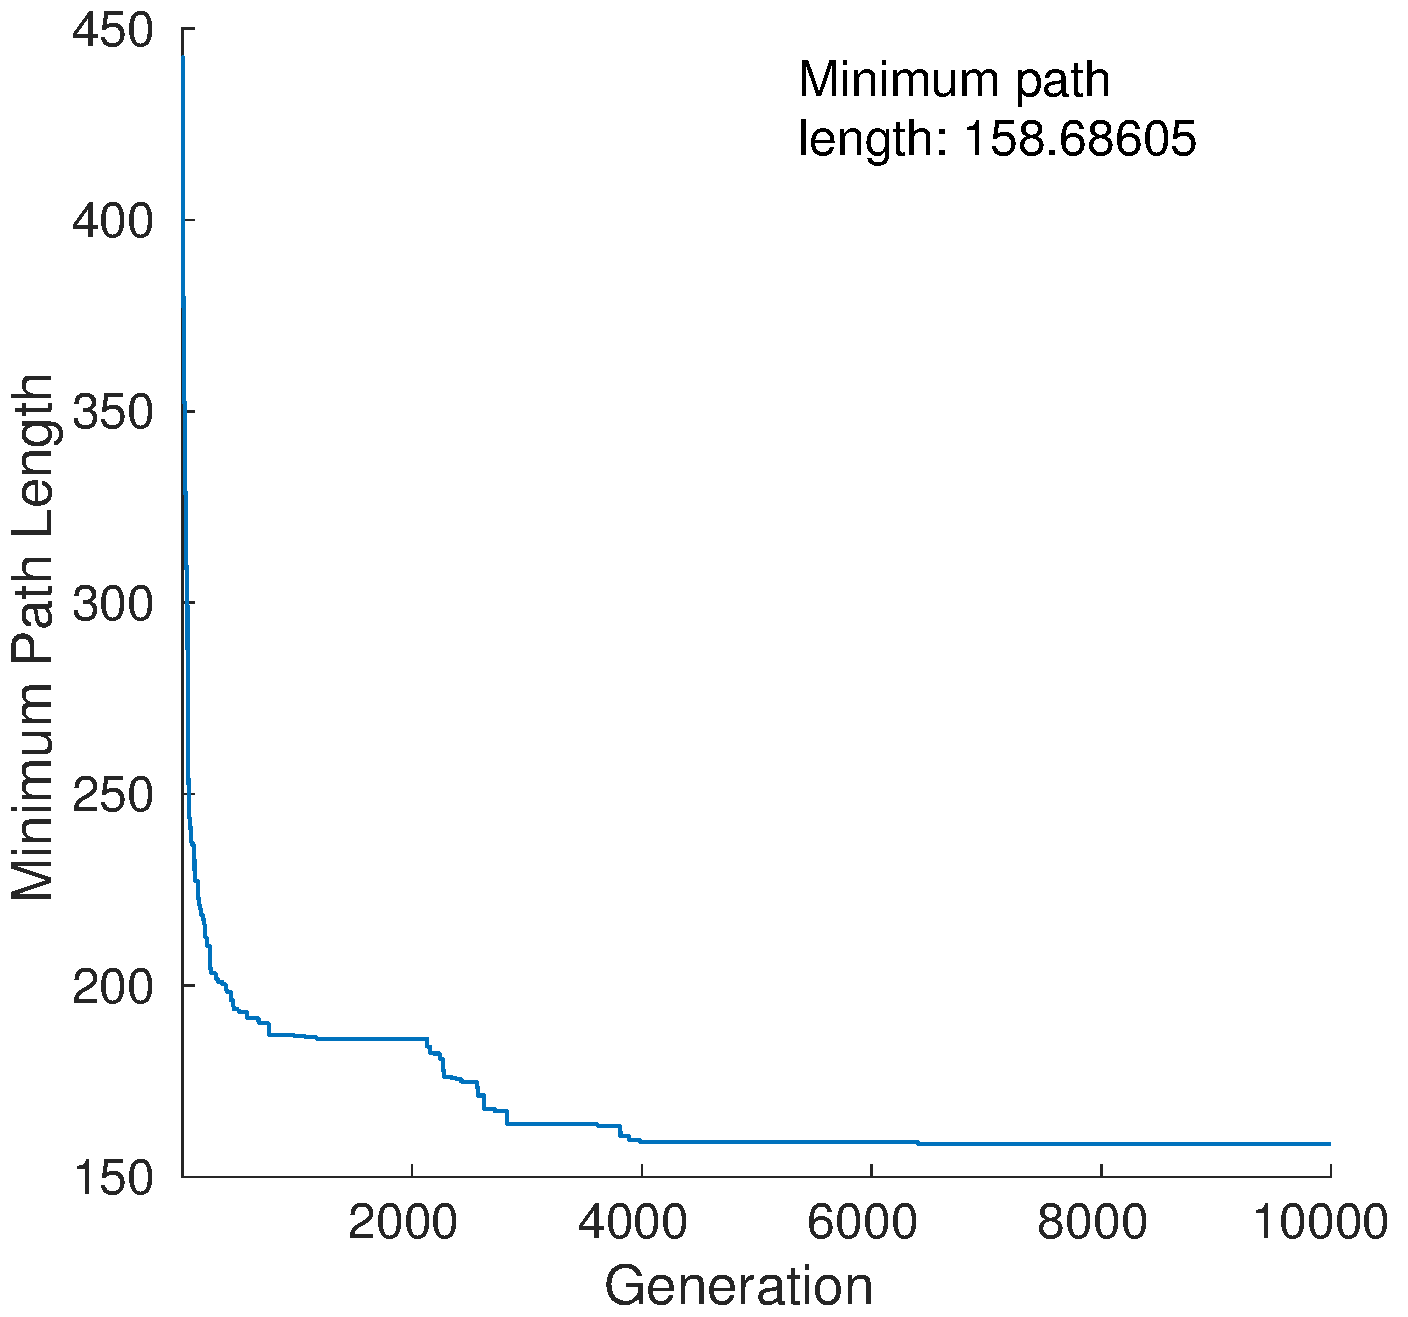
\includegraphics[width=\textwidth]{Figures/2b_minpathLength}
	\caption{}
	\label{subfig:2b_minPathLength}
\end{subfigure} %
\hfill %
\begin{subfigure}{0.45\textwidth}
	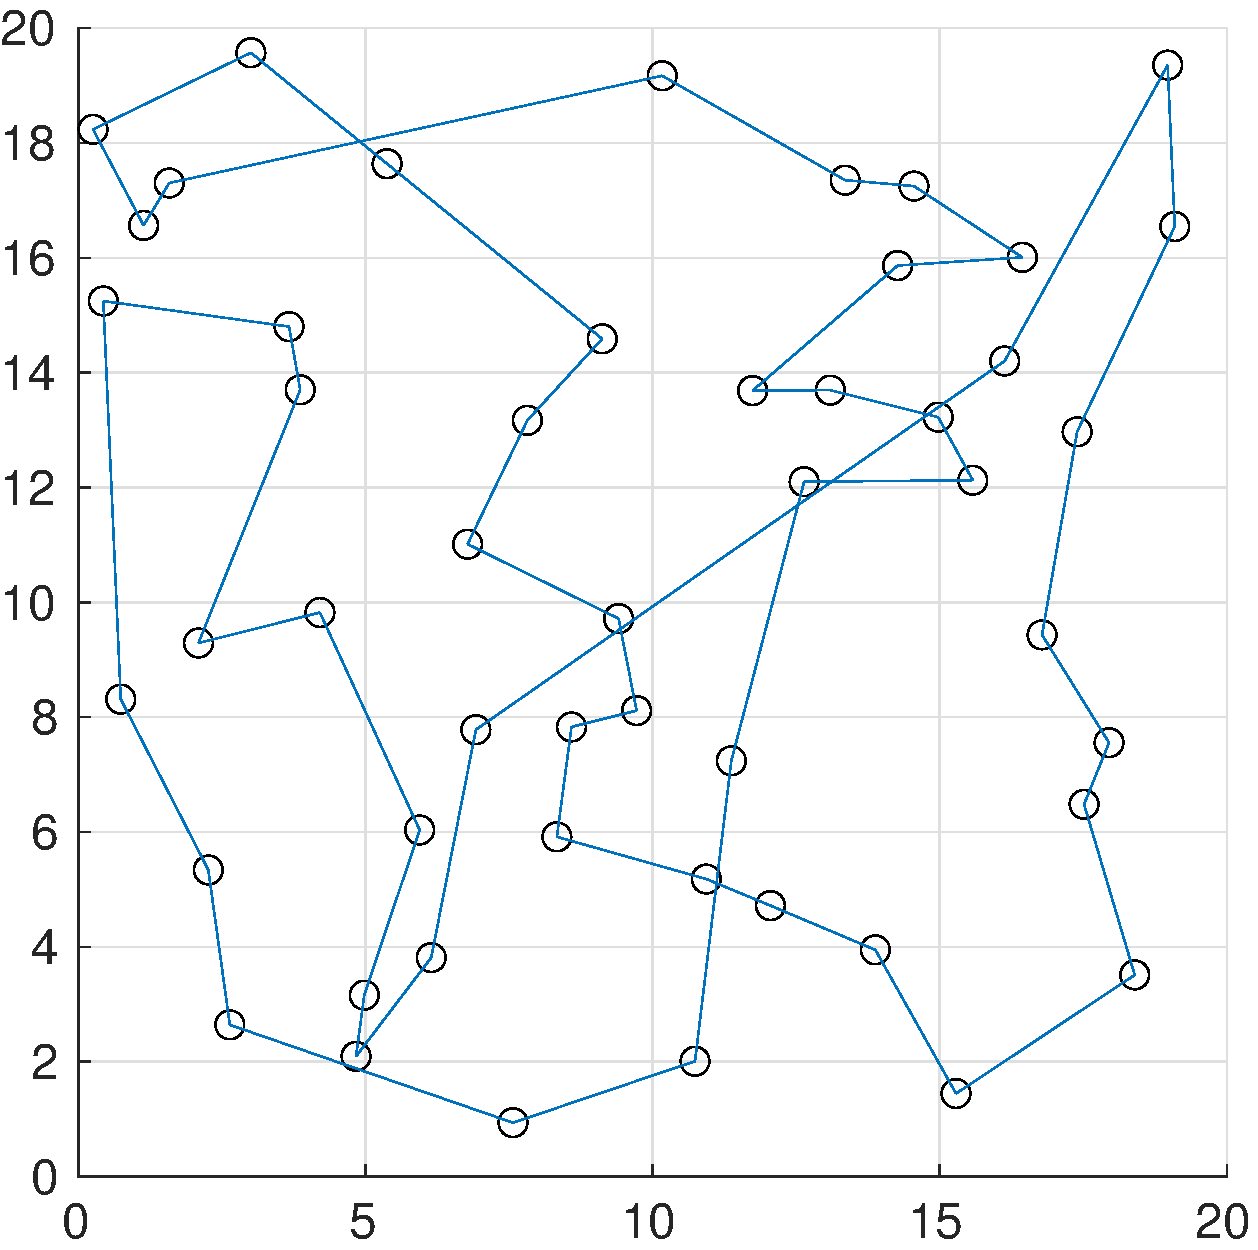
\includegraphics[width=\textwidth]{Figures/2b_pathPlot}
	\caption{}
	\label{subfig:2b_pathPlot}
\end{subfigure} %
\caption{\footnotesize Best result found by \texttt{GA21b.mat} (GA for TSP with random initial population). Left panel: minimum path length vs. generations. Right panel: best path found (length $\simeq$ 158.69).}
\label{fig:1b}
\end{figure}

\subsection*{2.1(c)}

An Ant System (AS) algorithm was implemented by completing the provided \textsc{matlab} script \texttt{AntSystem.m} and then applied to the same TSP as above. 

After experimenting with several parameter sets, it was found that using a larger number of ants than $N$ (number of cities) could help avoiding premature convergence, as more pheromone is deposited in each iteration. The path of length 122.44 shown in Figure~\ref{fig:1c} was obtained by running \texttt{AntSystem.m} with 100 ants and parameters $\alpha = 2, \ \beta = 1, \ \rho = 0.5$, after 107 iterations. The AS algorithm was thus able to find a better solution than the GA. The chromosome corresponding to this path is saved as a vector in file \texttt{bestPath21.m} (in main problem folder \texttt{2.1}), which can be run as a script and loads a vector called \texttt{bestPath} in the workspace.

\begin{figure}[htbp]
\centering
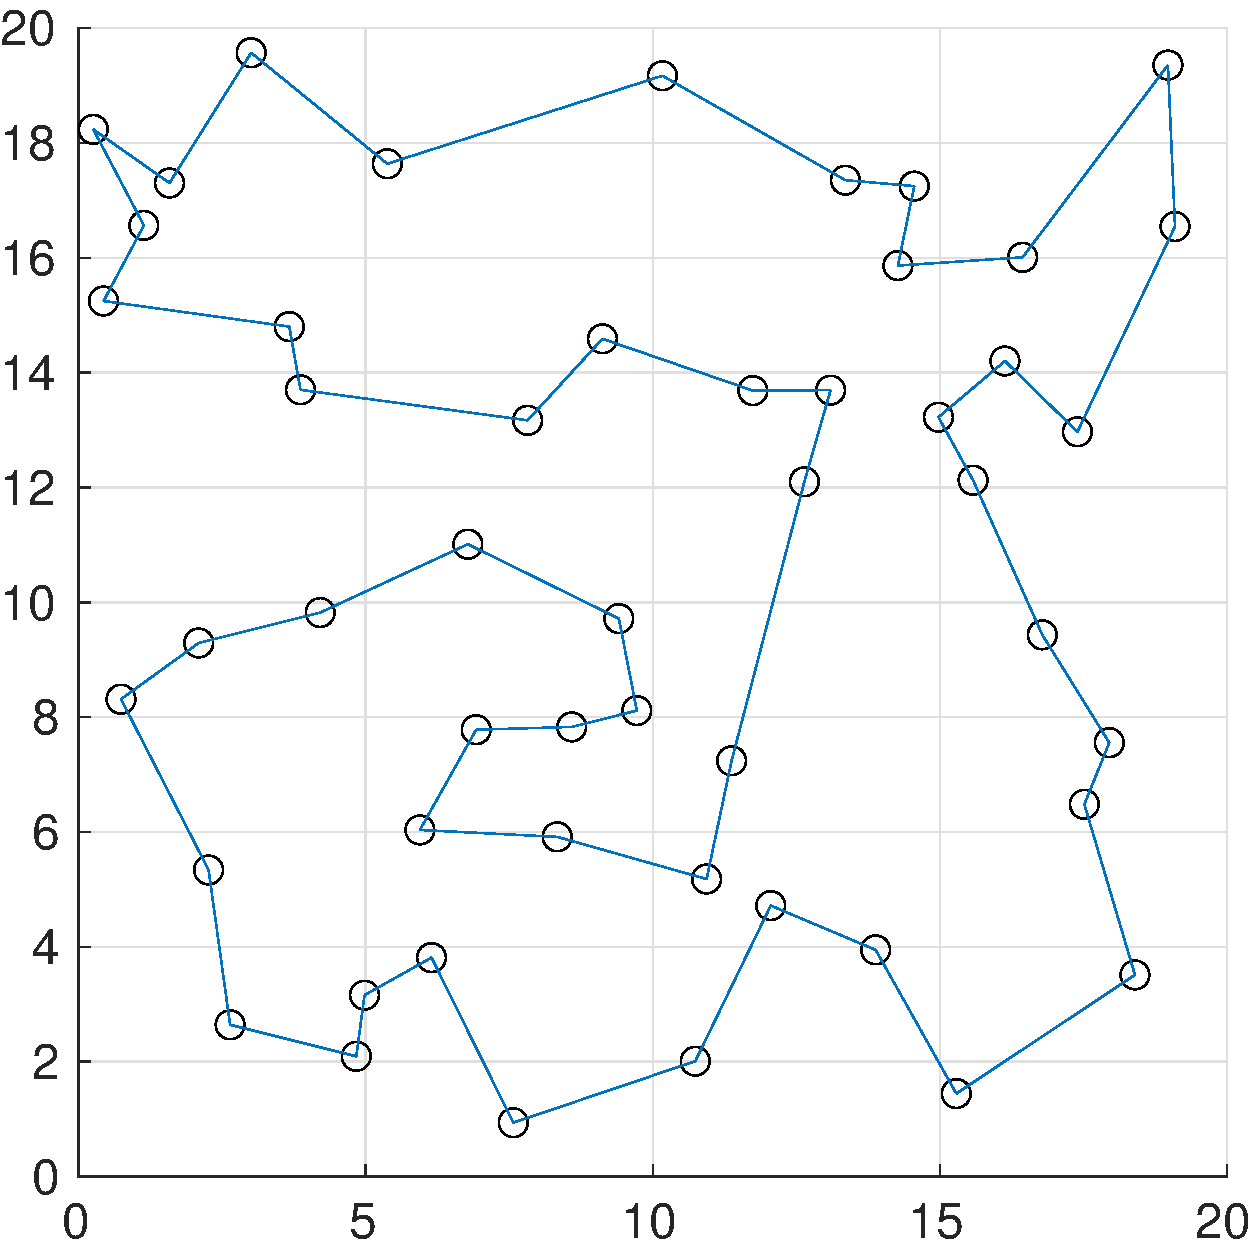
\includegraphics[width=0.45\textwidth]{Figures/2c_pathPlot}
\caption{\footnotesize Best path found with Ant System algorithm. Length $\simeq$ 122.44.}
\label{fig:1c}
\end{figure}

\subsection*{2.1(d)}
To allow a more fair comparison between GA and AS, the initialisation of the GA population was modified, so that starting path are nearest-neighbour paths (generated by starting from a random city) with a few random swap mutations (see function \texttt{InitializePopulation21d}).

Figure~\ref{fig:1c} shows the best result of a set of long runs (10000 generations) of the GA with 100 individuals and the same parameters as in 2.1(b), starting from a population of nearest-neighbour paths with 3 swap mutations each.
The length of the best path found by \texttt{GA21d.mat} was $130.76$. Thus, as expected, this implementation yields better results that the one in 2.1(b). However, AS implementation in 2.1(c) remains far superior for solving this combinatorial optimisation problem. 

\begin{figure}[htbp]
\centering
\begin{subfigure}{0.475\textwidth}
	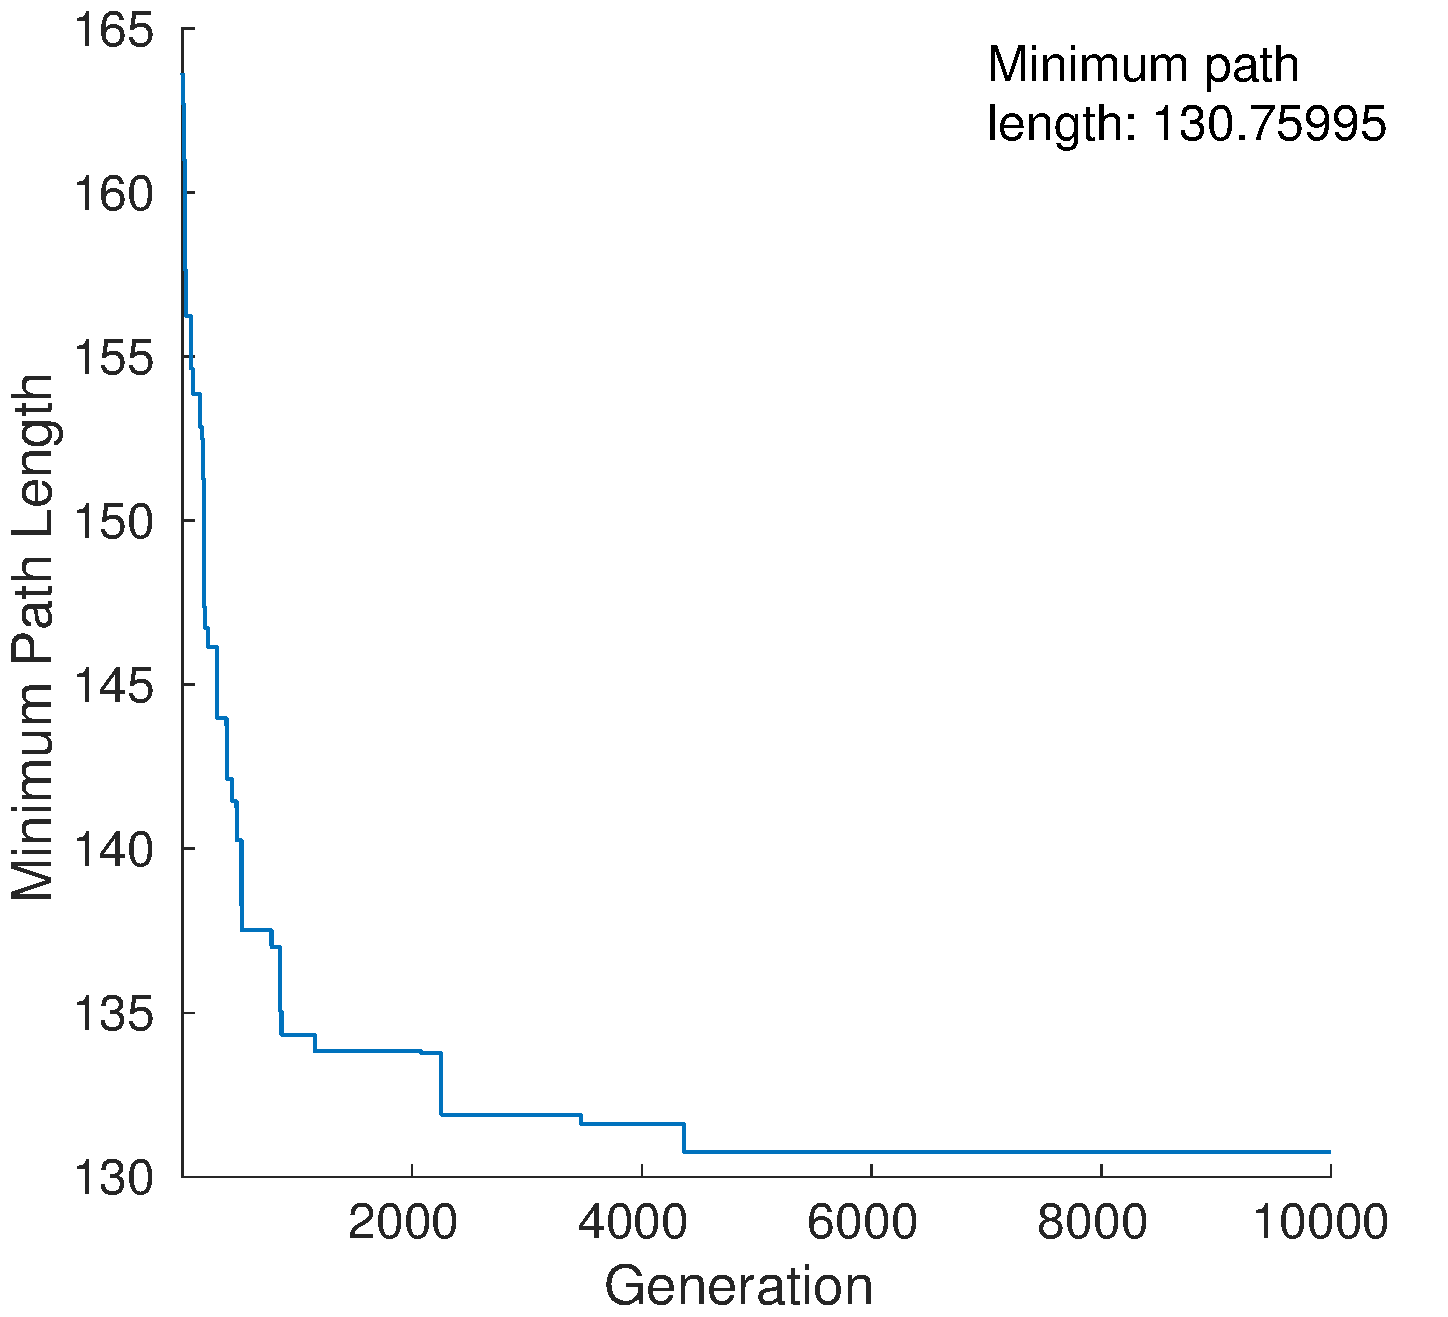
\includegraphics[width=\textwidth]{Figures/2d_minpathLength}
	\caption{}
	\label{subfig:2d_minPathLength}
\end{subfigure} %
\hfill %
\begin{subfigure}{0.475\textwidth}
	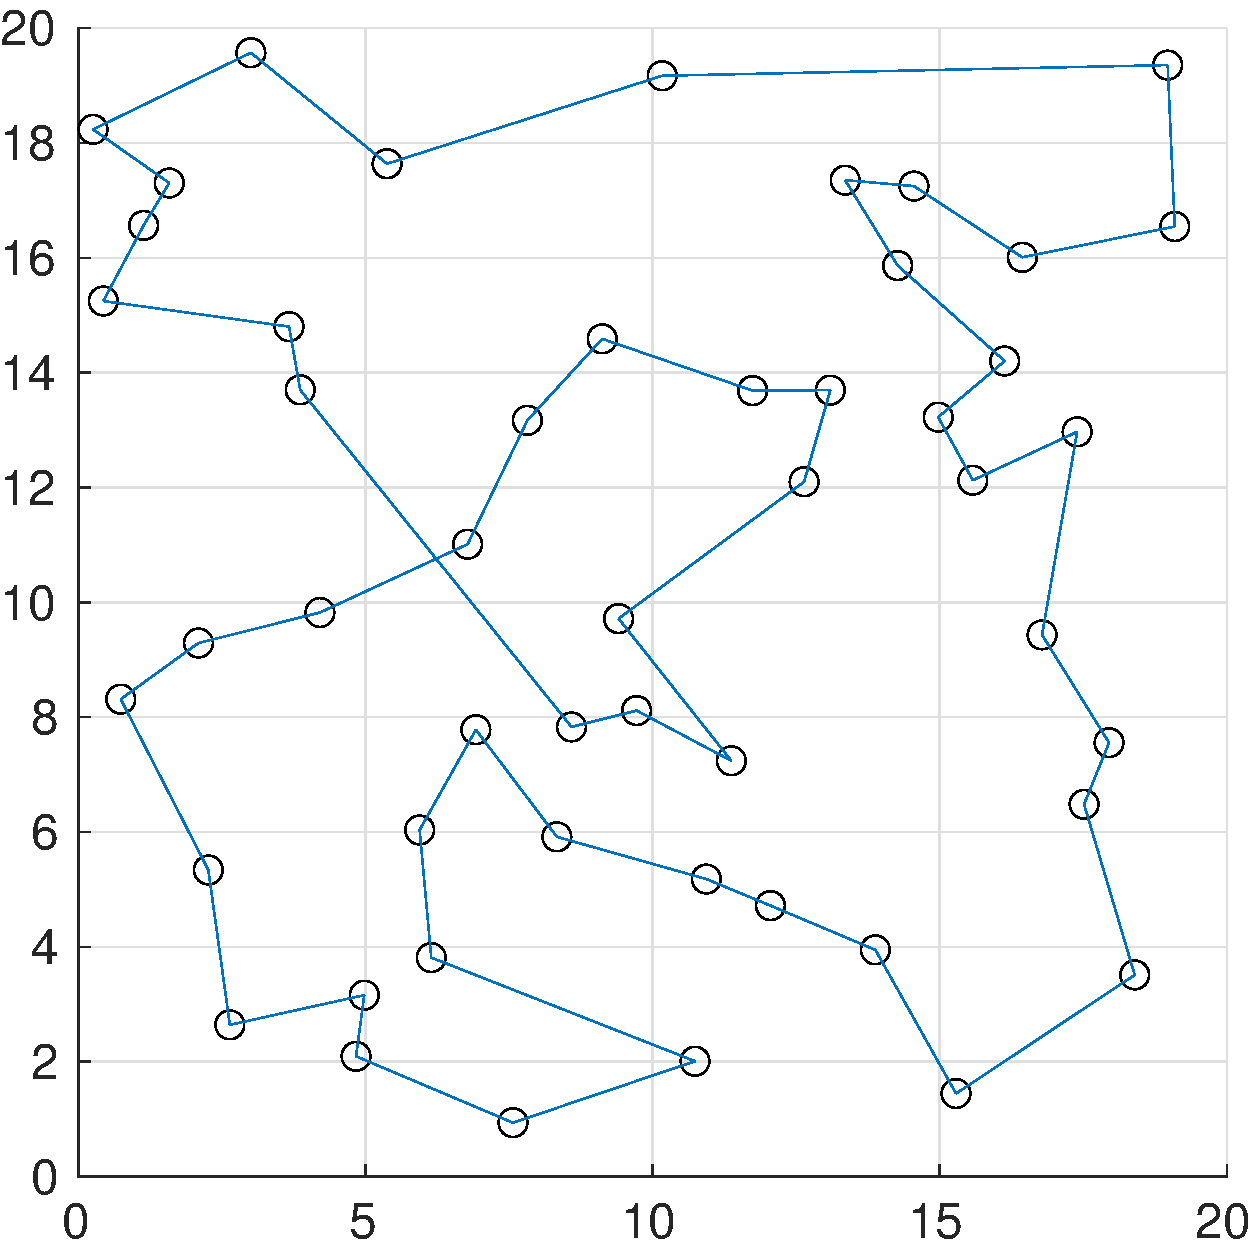
\includegraphics[width=\textwidth]{Figures/2d_pathPlot}
	\caption{}
	\label{subfig:2d_pathPlot}
\end{subfigure} %
\caption{\footnotesize Best result found by \texttt{GA21d.mat} (GA for TSP with initial population of nearest-neighbour paths with 3 swap mutations). Left panel: minimum path length vs. generations. Right panel: best path found (length $\simeq$ 130.76).}
\label{fig:1d}
\end{figure}

\section*{Problem 2.2 - Particle swarm optimisation}

\subsection*{2.2(a)}
\textsc{matlab} script \texttt{PSO22a} in folder \texttt{2.2/2.2a} contains an implementation of a standard PSO algorithm for function minimisation, with inertia weights and no craziness operator.

The program was used to find the minimum of the function
\[
f(x, y) = 1 + (-13 + x - y^3 + 5y^2 - 2y)^2 + (-29 + x + y^3 	+ y^2 - 14y)^2 \ ,
\]
with $x$ and $y$ real values in $[-10, 10]$. 

After a few runs to explore the parameter space, the parameter set in Table~\ref{tab:2a} was used to find the minimum
\[
(x^*,y^*)^T = (5, \ 4)^T \ , \qquad \mbox{with} \qquad f(x^*,y^*) = 1 \ .
\]

\begin{table}[hbtp]
\centering
\begin{tabular}{cccccccccc}
\toprule
Swarm & Number of &  &  &  &  & Maximum & Starting & Inertia weight & Minimum \\
size & iterations & $ \alpha$ & $ \delta t$ & $ c_1$ & $ c_2$ & speed & inertia weight & decrease rate & inertia weight \\
\midrule
20 & 1000 & 1 & 1 & 2 & 2 & 20 & 1.4 & 0.99 & 0.3 \\
\bottomrule
\end{tabular}
\caption{\footnotesize PSO parameters used in \texttt{PSO22a}.}
\label{tab:2a}
\end{table}

\subsection*{2.2(b)}
The PSO was then modified to handle integer programming (see script \texttt{PSO22b} in folder \texttt{2.2/2.2b}). When the objective function is evaluated, particle positions are temporarily rounded to the nearest integer values, whereas floating point values are using in all other stages of the computation.

The script was then used to find the minimum of the function
\[
f(\bm{x}) = -(15 \ 27 \ 36 \ 18 \ 12) \ \bm{x} + \bm{x}^T \ \begin{pmatrix}
35 & -20 & -10 & 32 & -10 \\
-20 &  40 & -6 & -31 & 32 \\
-10 & -6 & 11 & -6 & -10 \\
32 & -31 & -6 & 38 & -20 \\
-10 & 32 & -10 & -20 & 31 \\
\end{pmatrix} \ \bm{x} \ ,
\]
where $ \bm{x} = (x_1 , x_2 , x_3 , x_4 , x_5 )^T$, and $x_i \in \lbrace -30, -29, \ldots , 29, 30 \rbrace \in \mathbf{Z}$.

Using parameters in Table~\ref{tab:2b}, two (possibly global) minima were found:
\[
\bm{x^{*}}_{(1)} = (0, 11, 22, 16, 6)^T \ , \quad \mbox{and} \quad \bm{x^{*}}_{(2)} = (0, 12, 23, 17, 6)^T \ , \qquad \mbox{both with} \ f(\bm{x^*}_{(i)}) = -737 \ .
\]

\begin{table}[hbtp]
\centering
\begin{tabular}{cccccccccc}
\toprule
Swarm & Number of &  &  &  &  & Maximum & Starting & Inertia weight & Minimum \\
size & iterations & $ \alpha$ & $ \delta t$ & $ c_1$ & $ c_2$ & speed & inertia weight & decrease rate & inertia weight \\
\midrule
50 & 2000 & 1 & 1 & 2 & 2 & 60 & 1.4 & 0.99 & 0.3 \\
\bottomrule
\end{tabular}
\caption{\footnotesize PSO parameters used in \texttt{PSO22b} (integer programming).}
\label{tab:2b}
\end{table}

\section*{Problem 2.3 - Optimisation of braking systems}

An intelligent braking system for trucks descending slopes was developed by evolving populations of multilayer FFNN with three inputs (normalised velocity $v/v_{\textup{max}}$, slope $\alpha / \alpha_{\textup{max}}$ and foundation brakes temperature $T/T_{\textup{max}}$) and two outputs (brake pedal pressure $ P_p$ and requested gear change $\Delta_{\textup{gear}}$).

GA parameters and other parameters of the truck basic model can be specified at the beginning of the main script \texttt{BrakingSystemOptimisation.m} (in folder \texttt{2.3/GA\_Training}). The script generates a population of chromosomes representing (3-$N_h$-2)-perceptrons, where the number $N_h$ of hidden units can be modified by the user (hard-coded default value $N_h$ = 8), with genes sampled uniformly at random in [0,1] (real number encoding). Specifically, chromosomes are ($2\times1$) \textsc{matlab} cells containing two weight matrices (input-to-hidden and hidden-to-output), and each such matrix also includes neuron biases in an extra column.
 
At the evaluation step, each chromosome is decoded into the corresponding FFNN with rescaled weights and biases (default range [-10, 10]) and such network is then used as a braking control system, running a series of simulations on different slopes. Network outputs at each time-step are used to control the truck pedal pressure and gear. The gear, in particular, is increased by one if $\Delta_{\textup{gear}} > 0.7$, decreased by one if $\Delta_{\textup{gear}} < 0.3$ and otherwise left unchanged. Moreover, the gear value is only modified if no gear changes have occurred in the last 2 seconds.  

At the end of each simulation, the network fitness on the slope $i$ is calculated as
\[
F_i = \sqrt{\bar{v}_i \ d_i } \ ,
\]
where $\bar{v}_i$ is the average speed over the simulation (before termination), and $d_i$ is the travelled distance. Each simulation is stopped if any of the following constraints is violated:
\begin{itemize} \itemsep0em
\item $T > T_{\textup{max}}$ (maximum brakes temperature exceeded);
\item $v > v_{\textup{max}}$ (maximum speed exceeded);
\item $v < 0$ (truck stopped);
\item $d > d_{\textup{max}}$ (slope completed, where by default $d_{\textup{max}} = 1000$ m).
\end{itemize}
Simulations are performed on a set of 10 training slopes and on a set of 5 validation slopes\footnote{Training, validation and test slopes are generated using the provided slopes as templates and are hardcoded in function \texttt{GetSlopeAngle.m}}. At the end of each simulation set, the FFNN fitness is taken as 
the mean of the fitness values $F_i$. Only the fitness value computed on the training set is used as feedback for the GA, whereas the validation fitness is only used for determining when to stop the training process. The reference function for the evaluation step is \texttt{EvaluateNetwork.m}, which basically integrates the simple equation of motion of the truck described in the task. Model parameters are harcoded in the function, and were set to the suggested values, using SI units. The default time-step length $\Delta t$, instead, is $0.1$ s.

At the selection step, tournament selection is used (default parameters: size = 3 and ${p_{\textup{tour}} = 0.8}$). Crossover operator is not used, as neural networks perform distributed computation and crossbreeding two good networks does not necessarily produce a good offspring network (in fact, it usually does not).

Mutation operator works as follows: if a gene has to be mutated, i.e. a drawn random number is lesser than $p_{mut} $ (default value ${1/n_{\textup{genes}}} = {1/(6 N_h + 2) = 0.02}$), then another random number is drawn. If this number is lesser than $p_{\textup{creep}}$ (default value = 0.3), then a uniform creep mutation with rate $C_r$ (default value = 0.2) is applied to the gene, making sure it does not fall below 0 or rise above 1. Otherwise, the mutation is full-range, and the gene is set to a random value in [0,1].

At each generation, the network with the highest training fitness is copied unchanged in the next population (more than one copy can be replicated by modifying parameter \texttt{elitismCopies}).

\bigskip
Several training runs were carried out, with various parameters sets. A typical run is shown in Figure~\ref{fig:3_fitness}. Very long simulations were not possible due to a lack of time, therefore the overfitting phenomenon was not observed. Thus, in order to select the best network, in the final generation the networks with the highest fitness on the training and validation sets were compared by testing them on the (previously unseen) test set. The network with the highest fitness on the test set was taken as the best network \emph{of each run}. A set of 5 best networks were obtained with this procedure. The \emph{overall best} network was then chosen by comparing the fitness values of these 5 networks on the test set. The best o these 5 FFNNs was able to complete all 5 slopes in the test set without violating any temperature or speed constraint.

The \emph{best overall} network is hard-coded in the script \texttt{TestProgram.m}, in folder \texttt{2.3/Test\_Program}. This script allows to rerun the network on an arbitrary slope, which must be specified in the beginning of the script as an anonymous \textsc{matlab} function, as in\\
\hspace*{3cm} \texttt{alpha = @(x) 4 + sin(x/50) - 2*cos(sqrt(3)*x/50);}

\begin{figure}[htbp]
\centering
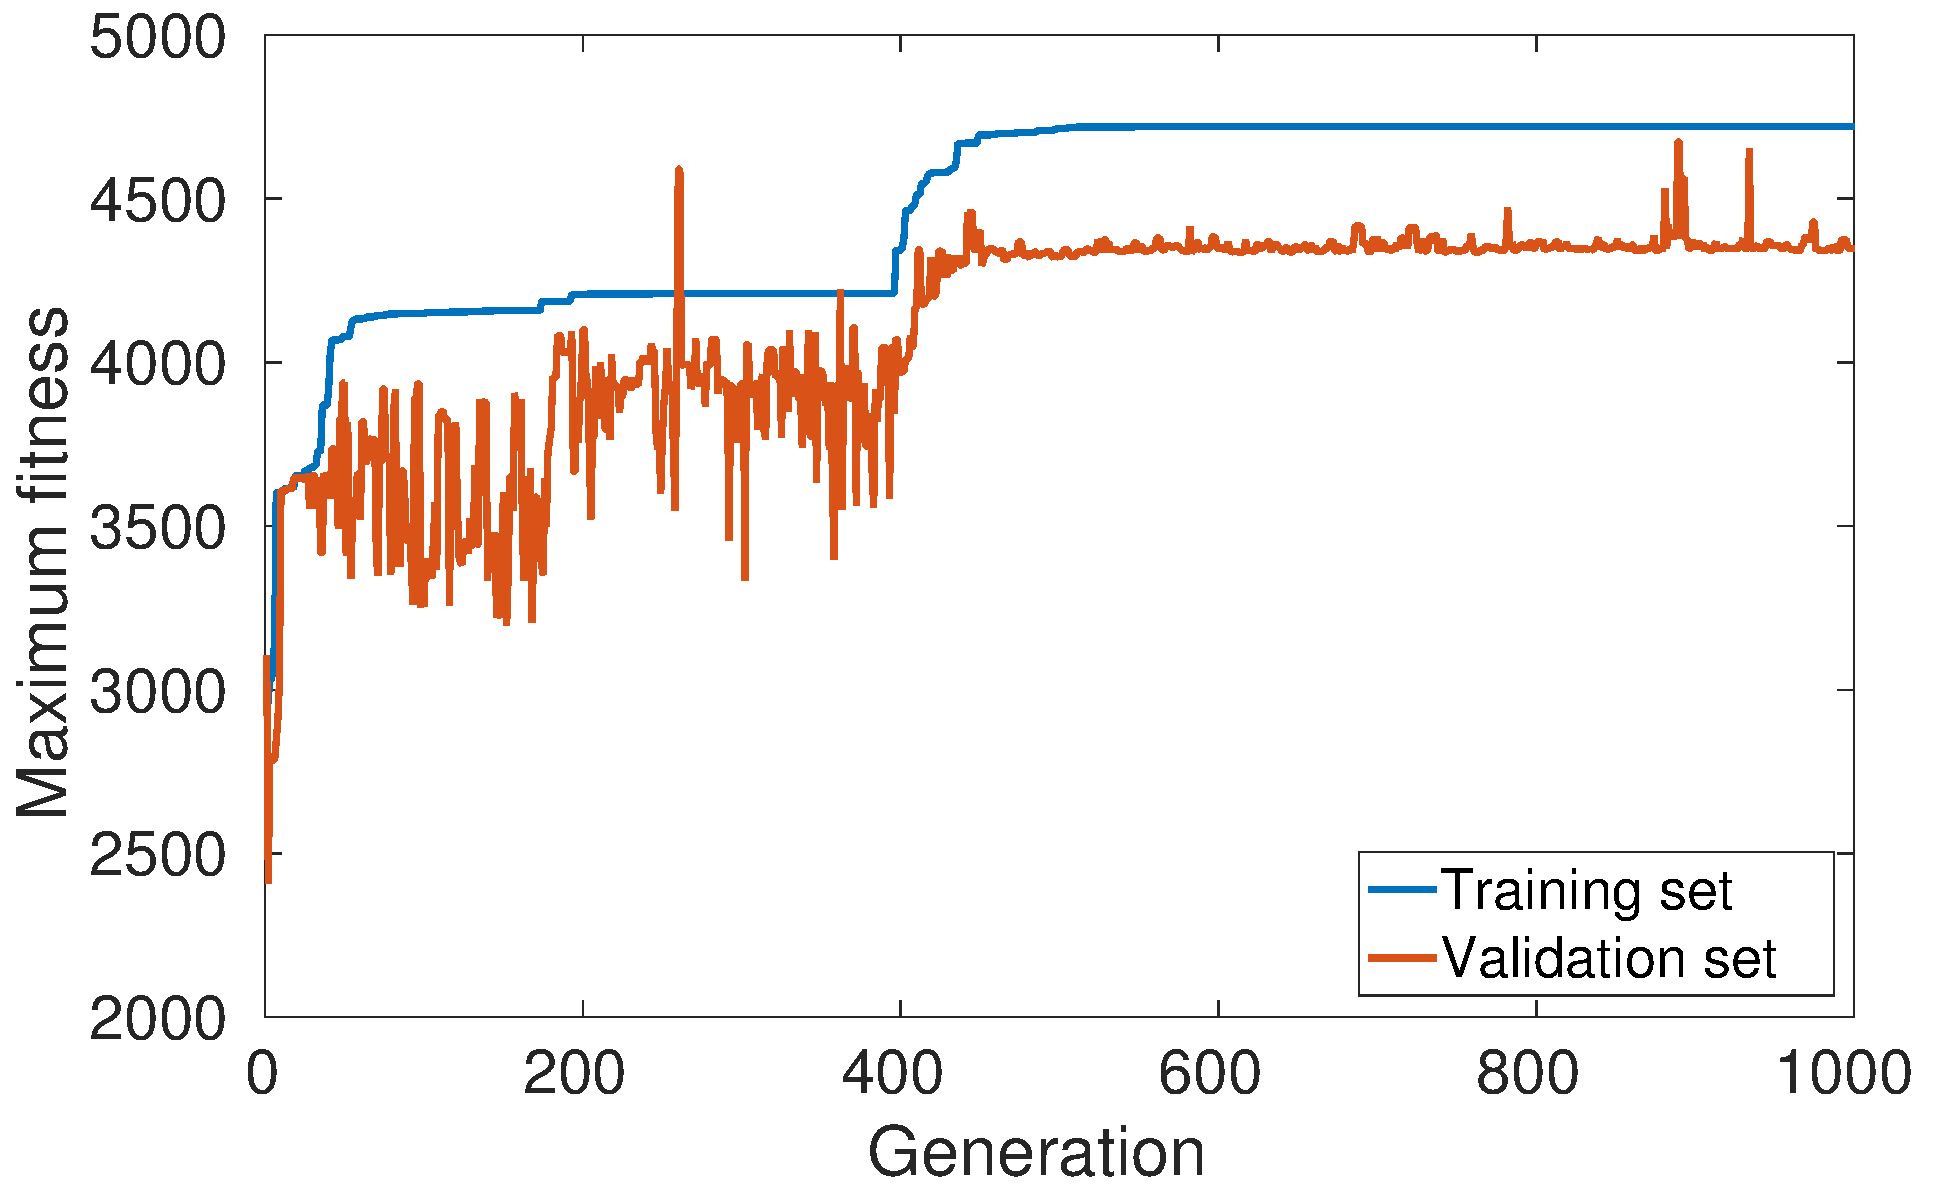
\includegraphics[width=0.55\textwidth]{Figures/3_fitness}
\caption{\footnotesize Maximum fitness in the population in a typical training run. Training set in blue, validation set in red.}
\label{fig:3_fitness}
\end{figure}

\vspace*{-1cm}
The (horizontal) length of the slope can also be specified at the beginning of the script, by modifying variable \texttt{slopeLength} (default value = 1000). Other parameters can also be modified, but this can affect the performance of the network, as the training process was carried out with the hard-coded default parameters.
At the end of the run, the script plots some graphical outputs showing the FFNN performance as an intelligent braking system. Figure~\ref{fig:3_performance} shows the performance of the best network found tested on the slope above (taken from the test set) extended to $10000$ m. As we can see, the truck is able to complete the (rather lengthy) run without brake overheating or exceeding the maximum speed.

%\vspace*{-0.2cm}
\begin{figure}[H]
\centering
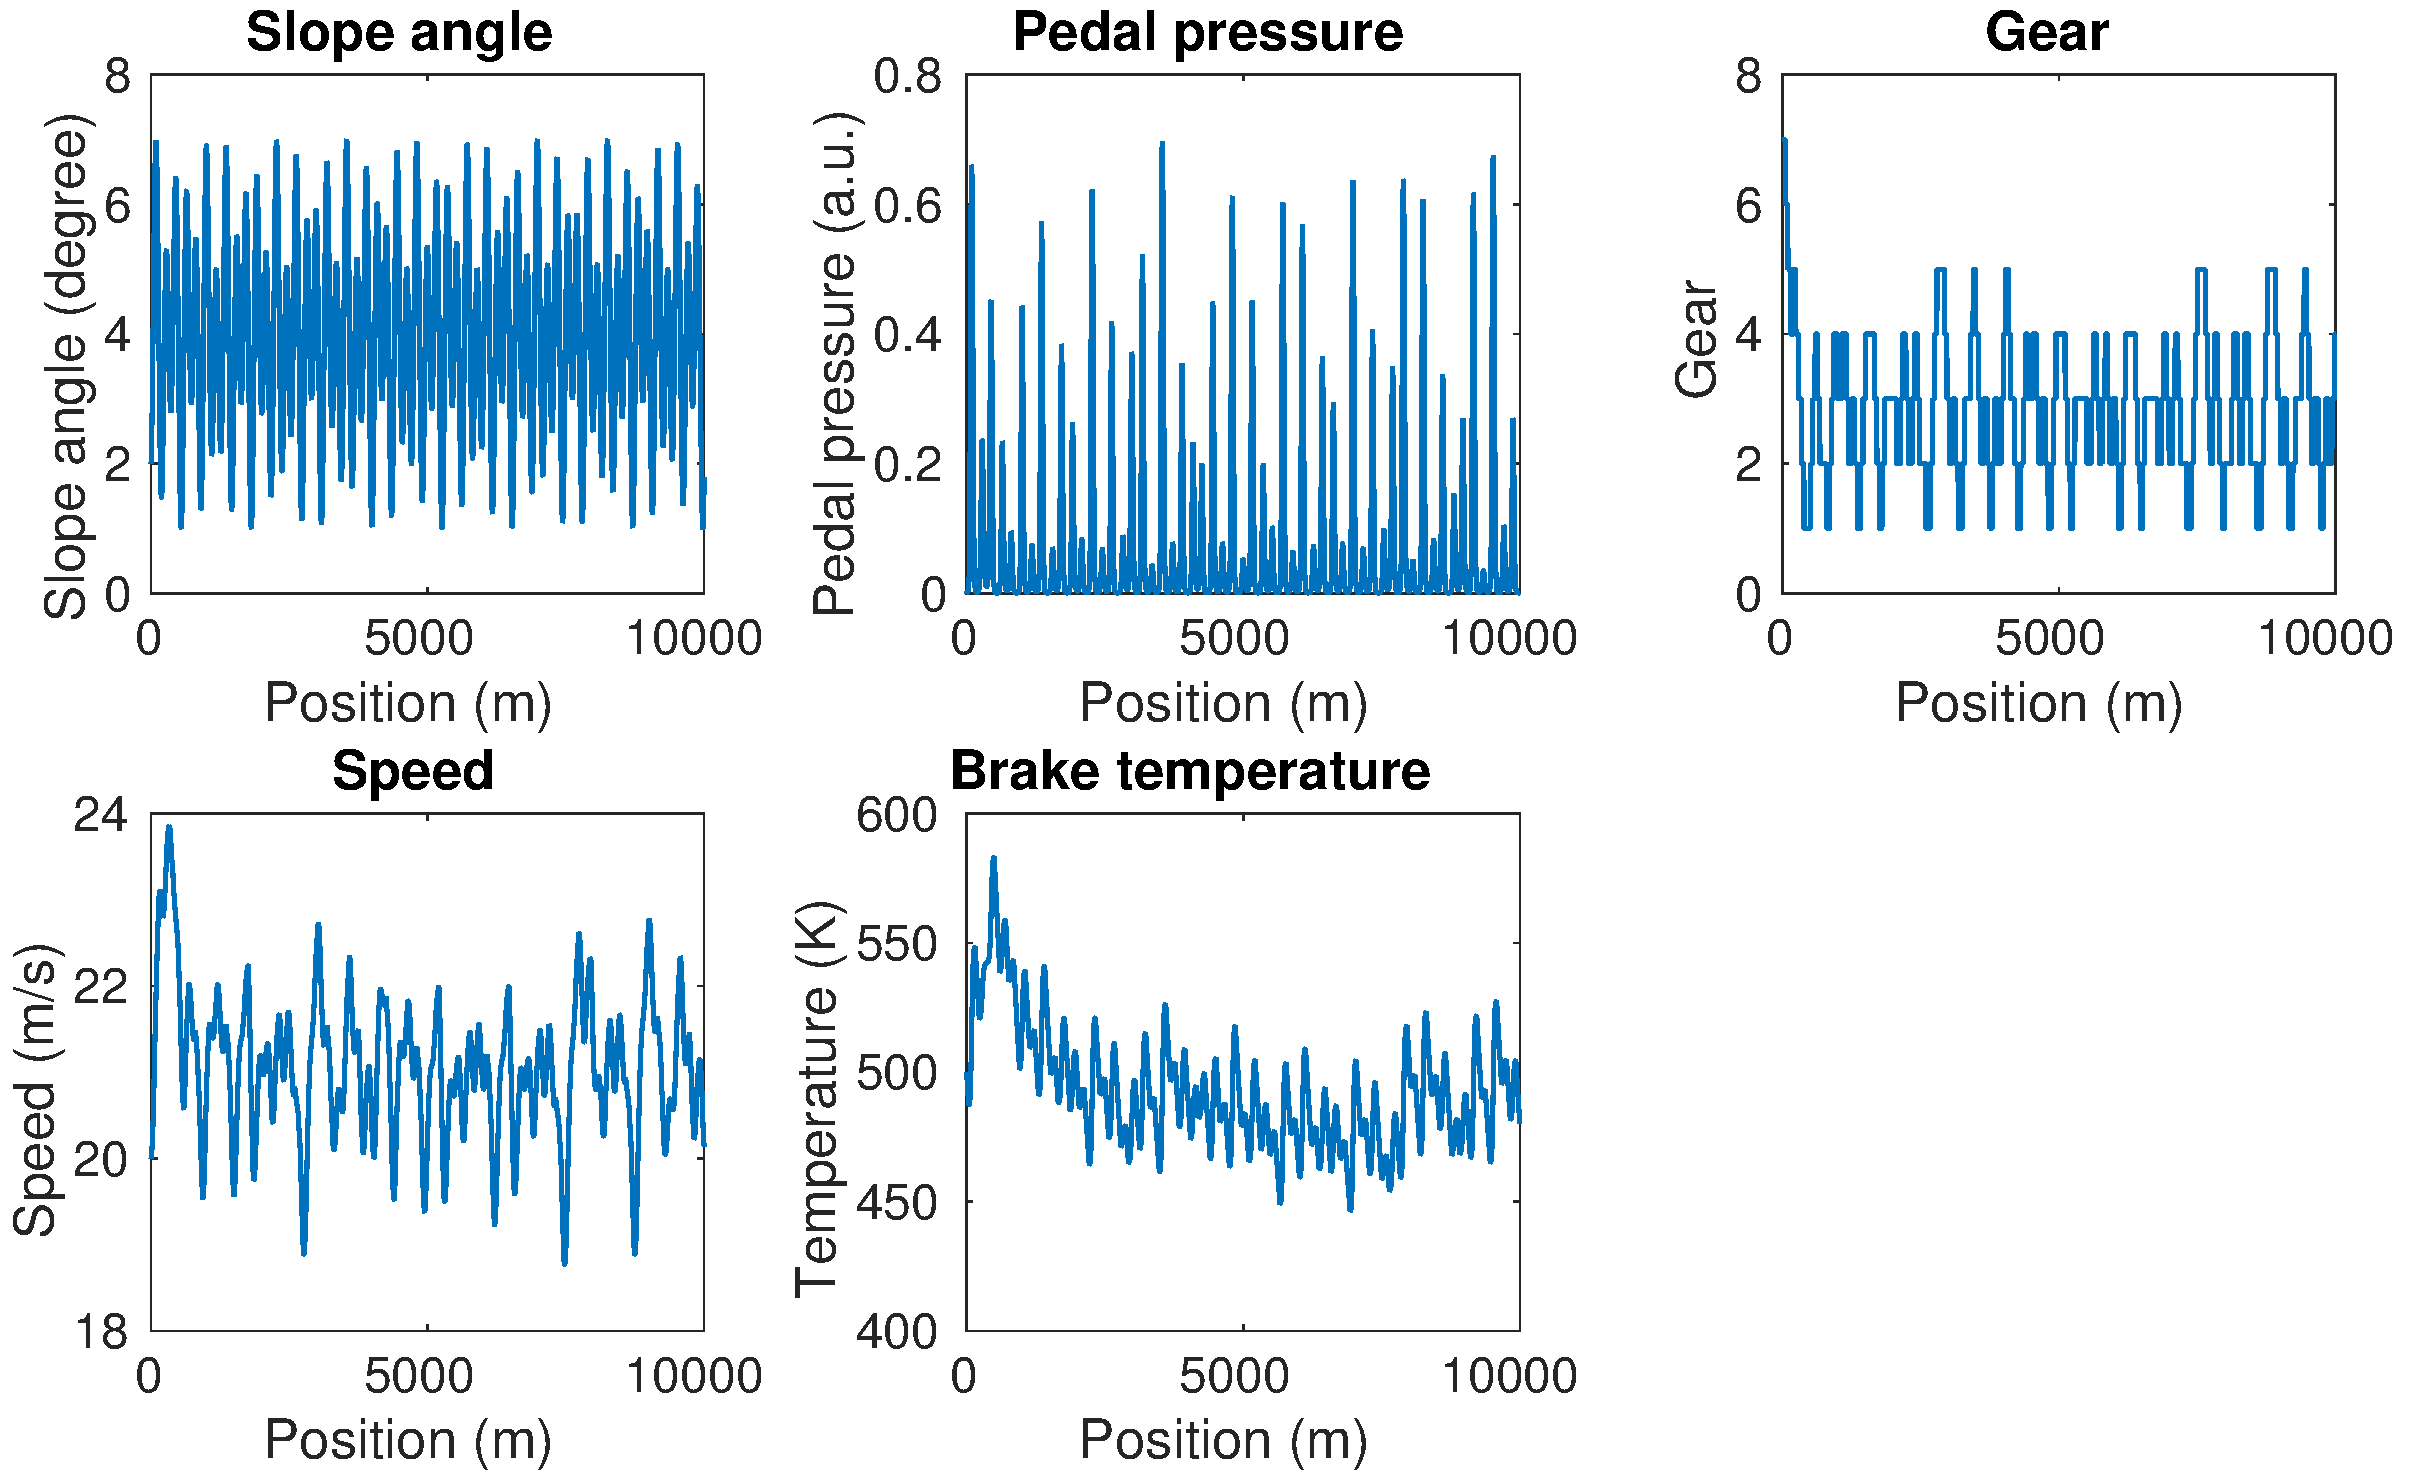
\includegraphics[width=\textwidth]{Figures/3_performance}
\caption{\footnotesize Performance of the FFNN hard-coded in script \texttt{TestProgram.m} on a slope picked from the test set.}
\label{fig:3_performance}
\end{figure}

\section*{Problem 4.4 - Function fitting using LGP}

A LGP program was implemented in \textsc{matlab}, to evolve functions fitting a given data set (see script \texttt{LGP24.m} in folder \texttt{2.4/LGP}).

First, a population of chromosomes representing sets of instructions is initialised. Each chromosome is a [$n \times 4$]-matrix, with $n$ being the number of instructions encoded in the chromosome. Each matrix entry is an integer value picked uniformly at random in its appropriate range, i.e. [1, 4] for the operator in column 1, [1,$\ M$] for the destination in column 2, [1,$\ M+N$] for the operands in column 3 and 4, where $M$ is the number of variable registers and $N$ is the number of constant registers. Only basic operators $\lbrace +, -, \times, / \rbrace$ are used in the program, and division is protected with constant $c_{\textup{max}}$.

Given a data set of $K$ values $(x, y)$, the program places a value $x_k$ in the first variable register $r_1$, whereas all other variable registers are set to 0, then the instructions encoded in the chromosome are evaluated and the final value of $r_1$ is used as the output, i.e. the function estimate $\hat{y}_k$ of $y_k$. This is repeated for each $k = 1,\ldots,K$. The chromosome fitness is then taken as the inverse of the error defined as
\[
e = \sqrt{\dfrac{1}{K} \ \sum_{k=1}^K \ ( \hat{y}_k - y_k)^2} \ .
\]
The algorithm then proceeds with tournament selection, two-point crossover and mutation. Given two selected chromosomes, two-point crossover is carried out by cutting each of chromosome into 3 sub-matrices and then swapping the middle sub-matrices.
Mutation, instead, is carried out by checking each gene for mutation and, in case of success, by drawing an integer value uniformly at random in the corresponding range of the gene (see above-mentioned ranges). 

\bigskip
The program was used to find the curve which best fits the provided data set. Several runs were carried out with different parameters, in order to find a suitable parameter set for the problem. Finally, a few long runs were performed with the parameters in Table~\ref{tab:4_parameters}, finding a function yielding an error of $0.0169$. The best (though overly complicated) fitting function found is
\[
f(x) = \dfrac{-6 \ (- x^{17} + 7 x^{16} - 44 x^{15} + 184 x^{14} - 668 x^{13} + 1936 x^{12} +}{6 x^{18} - 37 x^{17} + 231 x^{16} - 900 x^{15} + 3192 x^{14} - 8748 x^{13} + 21696 x^{12} + } \ldots \qquad \qquad \qquad \qquad
\]
\[
\ldots \dfrac{- 4910 x^{11} + 10369 x^{10} - 19175 x^{9} + 29414 x^{8} - 38832 x^{7} + 40044 x^6 +}{- 43830 x^{11} + 81045 x^{10} - 123363 x^9 + 176566 x^8 - 206592 x^7 + 244500 x^6 +} \ldots
\]
\[
\qquad \qquad \qquad \qquad \qquad \qquad \ldots \dfrac{- 32814 x^5 + 13302 x^4 + 3294 x^3 - 18387 x^2 + 14094 x - 10935)}{- 228150 x^5 + 250542 x^4 - 182682 x^3 + 188325 x^2 - 79218 x + 64881} \ .
\]

This function is hard-coded in script \texttt{TestFit.m} (in folder \texttt{2.4/Test\_Fit)}, which can be run standalone to produce the plot in Figure~\ref{fig:4_fit}, showing the original data together with the best fitting curve found with LGP. The program also computes the fitting error and outputs it on the console.

\begin{table}[hbtp]
\centering
\begin{tabular}{ccc}
\toprule
Population size  			& $\qquad$ & 100 \\
Number of generations			& 	& 5000\\
Tournament size					& 	& 5 \\
$p_{\textup{tour}}$					& & 0.75\\
$p_{\textup{cross}}$				& & 0.2\\
$p_{\textup{mut}}$					& & 0.01\\
Number of variable registers $M$	& & 3\\
Number of constant registers $N$	& & 3\\
Constant registers values			& & (1, 3, -1)\\
Initial number of instructions	& 	& $5\sim 25$\\
$c_{\textup{max}}$				& 	& $10^{10}$\\
\bottomrule
\end{tabular}
\caption{\footnotesize Parameters used in LGP long runs.}
\label{tab:4_parameters}
\end{table}

\begin{figure}[hbtp]
\centering
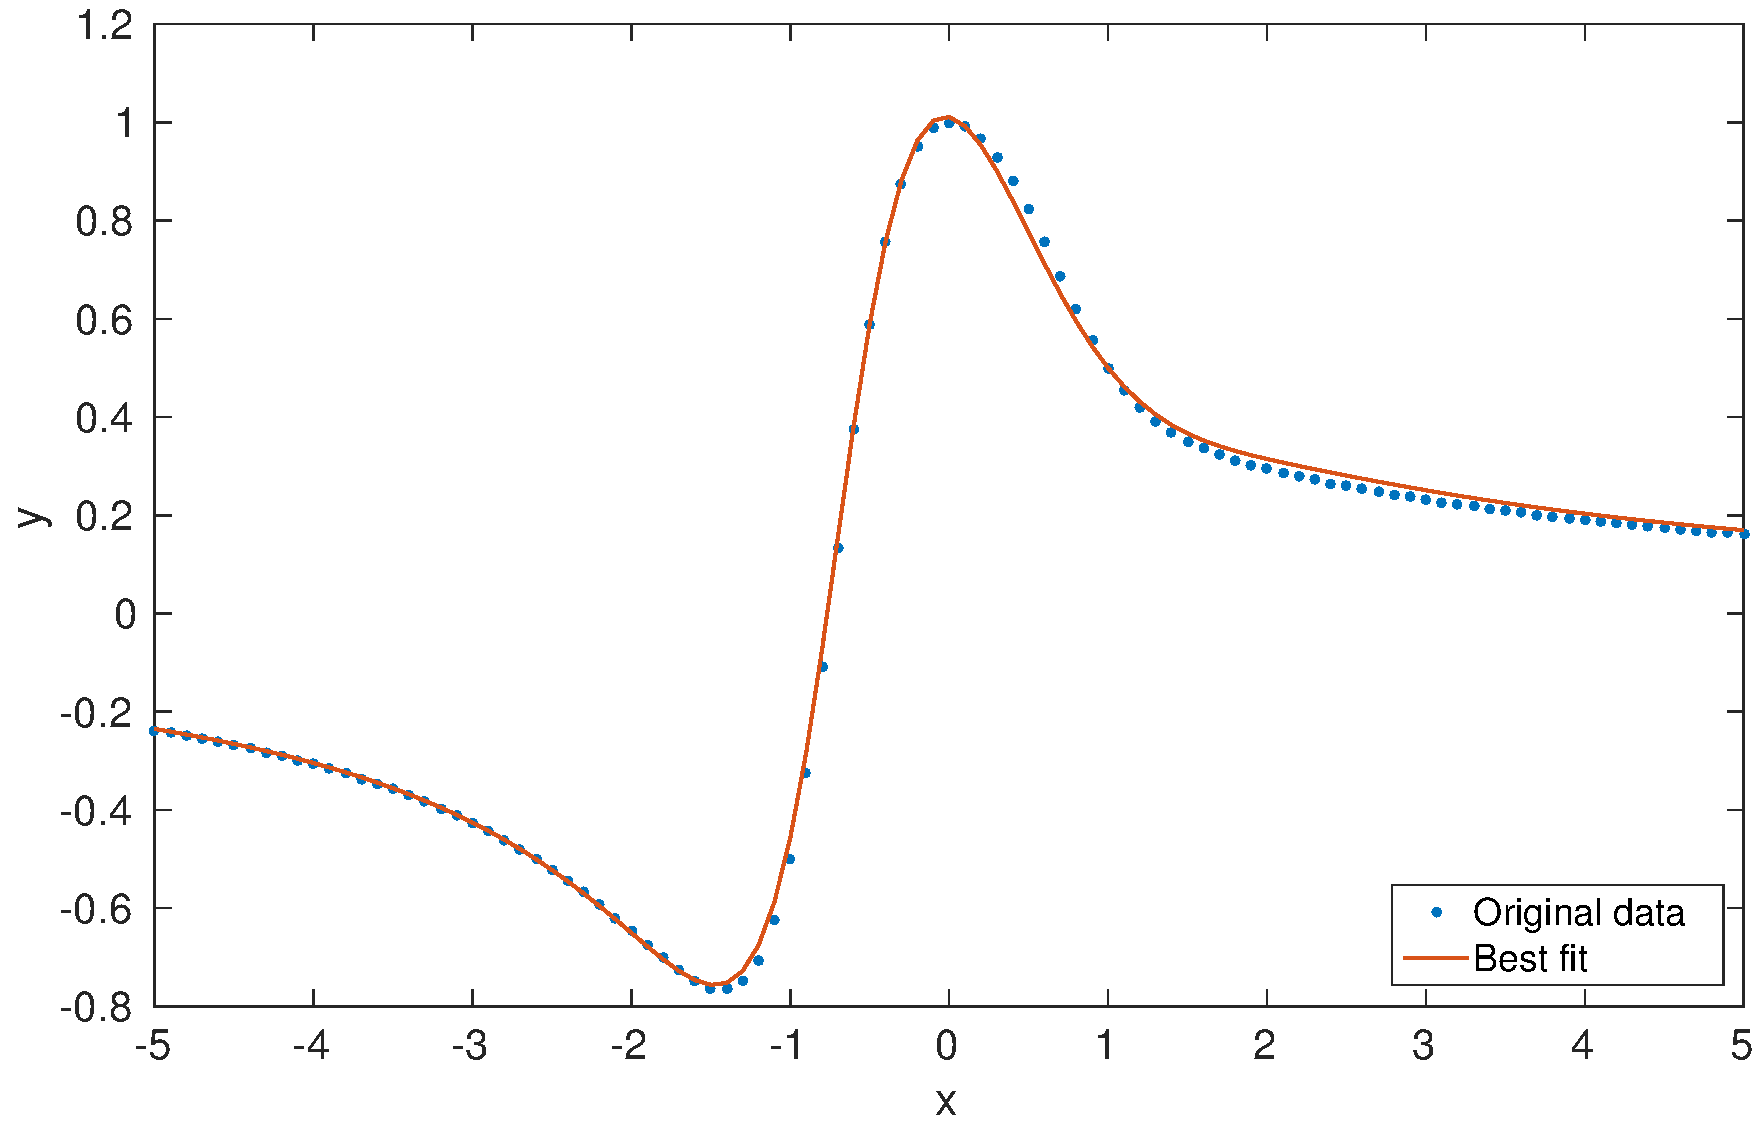
\includegraphics[width=0.9\textwidth]{Figures/4_fit}
\caption{\footnotesize Graphical output of program \texttt{TestFit.m}. Blue dots: original data points. Red curve: best fitting function found with program \texttt{LGP24.m}}
\label{fig:4_fit}
\end{figure}

\end{document}

